\documentclass{article}
\usepackage[utf8]{inputenc}
\usepackage[T1]{fontenc}
\usepackage{amsmath,amssymb,graphicx,hyperref,longtable}
\usepackage[margin=2.4cm]{geometry}
\title{Banking Intent Classification with Word and Character TF-IDF}
\author{Alex Dems}
\date{September 2026}
\begin{document}\maketitle
Alex Dems | NLP Course Final Project | September 2026

\section*{Abstract}
We study a lightweight classifier for 77 banking intents using BANKING77. The method concatenates word and character TF-IDF vectors and trains a linear support vector machine. A controlled feature ablation evaluates three training-data caps over three random seeds, followed by a larger training-pool experiment. On the official test set, the combined model reaches 90.91\% accuracy and 90.92\% macro-F1, compared with 88.12\% accuracy for word features alone. The experiments examine how the benefit of combining the two feature types changes with the amount of training data.

Project code accompanies this report in banking77\_project.zip. The repository URL is supplied separately in the course submission field.

\section*{1 Introduction}
Banking support systems must route short user messages to the correct action. Closely related requests, such as a delayed card and an estimated delivery time, make this a fine-grained language classification problem. A linear classifier is a useful baseline here: it is fast to train and its features can be inspected directly.

This study tests whether character n-grams improve a word-based classifier when training examples are limited. Word n-grams retain local phrases; character n-grams share information across related spellings and word forms. The hypothesis is that these representations complement each other. All features are learned from BANKING77; no external training data are used.

\subsection*{1.1 Team}
Alex Dems. Individual project: data preparation, implementation, experiments and analysis.

\section*{2 Related Work}
Wang and Manning [1] demonstrate that feature choice and linear-model variants can strongly affect text classification. Their NB-SVM uses supervised log-count-ratio features; our method uses ordinary TF-IDF and does not reproduce NB-SVM. Their findings motivate a careful lexical baseline, but sentiment classification scores are not directly comparable with banking-intent accuracy.

BERT [2] learns bidirectional contextual representations through pretraining, followed by task adaptation. Unlike our sparse model, it can represent a word differently across contexts. Sentence-BERT [3] adapts transformer encoders to obtain sentence representations through siamese/triplet training, enabling efficient embedding-based comparison. These are relevant semantic alternatives; we do not run them in this CPU-only study.

\clearpage
\section*{2 Related Work (continued)}
Casanueva et al. [4] introduced BANKING77 and compared fixed sentence encoders with fine-tuned BERT. Their Table 3 reports 93.66\% accuracy for BERT-TUNED and 93.36\% for USE+ConveRT with full training data; the latter obtains 85.19\% with 10 examples per intent. They provide reference points, although their training protocol differs from the validation split and sampling used here.

SetFit [5] adapts a sentence transformer using contrastive text pairs and then trains a classification head. Unlike TF-IDF, it starts with pretrained semantic representations. A comparison with SetFit would help separate the effect of feature choice from the benefit of pretraining; it is outside the experiments reported here.

\section*{3 Model Description}
The main model has two parallel feature branches. The word branch extracts unigrams and bigrams, capped at 50,000 features. The character branch extracts within-word character n-grams of lengths 3 to 5, capped at 80,000 features. Lowercasing is enabled; stop-word removal, stemming and lemmatization are disabled. The word branch uses the scikit-learn default token pattern (tokens with at least two word characters). The character branch uses char\_wb, including boundary padding.

Each branch uses sublinear term frequency and smoothed inverse document frequency. For a feature t appearing f(t,d) times in document d, tf = 1 + ln(f) for f > 0 and zero otherwise. With N training documents and document frequency df(t), idf(t) = ln((1 + N)/(1 + df(t))) + 1. TF-IDF is the product of these quantities, followed by L2 normalization. Vocabulary and IDF are learned only from the current training subset.

Let w(d) and c(d) be the two normalized sparse vectors. The combined representation is x(d) = normalize([w(d); c(d)]). When both branches are nonzero, this gives each branch equal norm. A second normalization prevents the concatenated vector from simply having a larger norm than a single-branch baseline.

A one-vs-rest LinearSVC classifier learns 77 linear decision functions. For each binary problem it minimizes L2 regularization plus C times the squared hinge loss. Prediction is argmax over the class decision scores. We use C = 1, tolerance 0.0001, dual optimization and at most 5,000 iterations. Scores are margins, not calibrated probabilities. Removing either feature branch produces the ablation baselines, while all classifier settings remain identical.

\section*{4 Dataset}
We use the public English BANKING77 dataset [4, 6], downloaded from the authors' repository. Its license is CC BY 4.0; attribution and the license text are included with the data snapshot. The original intent labels are used without additional annotation.

\begin{longtable}{p{4.83cm}p{4.83cm}p{4.83cm}}
Data partition & Examples & Role \\
Official train & 10003 & Source of all training/validation data \\
Cleaned official train & 9999 & After training-only deduplication \\
Training pool & 7999 & Model fitting and nested subsampling \\
Validation & 2000 & Held out; diagnostic evaluation only \\
Official test & 3080 & Fixed final comparison \\
\end{longtable}
Normalization for duplicate detection consists of lowercasing and whitespace collapsing. We remove 4 duplicate training rows; no conflicting normalized texts are found in train. A fixed stratified split reserves 20\% for validation. The training pool has 28 to 149 examples per class, while test contains 40 per class. Mean whitespace-token length is 11.95 in official train and 10.95 in test. Exact row indices and file SHA-256 hashes are saved.

\clearpage
\section*{5 Experiments}
\subsection*{5.1 Metrics}
Accuracy = (number of correct predictions) / N. For class k, F1(k) = 2 TP(k) / (2 TP(k) + FP(k) + FN(k)); macro-F1 is the arithmetic mean across all 77 classes. Accuracy is directly interpretable on the balanced official test set, while macro-F1 also reflects classwise precision/recall differences. All result tables express these metrics as percentages.

Reported standard deviations are sample standard deviations across training-subset seeds, not standard errors or confidence intervals. A paired bootstrap additionally resamples the 3,080 test rows 2,000 times and estimates the 2.5th/97.5th percentiles of the combined-minus-word accuracy difference. This interval is conditional on the fitted models and does not quantify training-set or domain-shift uncertainty.

\subsection*{5.2 Experiment Setup}
The split seed is 2026. For each cap in \{10, 30, 60\}, examples within each class are shuffled with seeds \{42, 43, 44\}; the first min(cap, available) rows are retained. The same rows are used by all three methods, and subsets are nested across caps within a seed. Rare classes are not oversampled. These caps give 770, 2,308 and 4,537 training examples, respectively; therefore only the 10-example regime is exactly balanced.

A further experiment uses all 7,999 training-pool rows once, with seed 42. There are 30 model fits in total: 3 methods x 3 caps x 3 seeds, plus 3 pool fits. The pool condition is not the complete official training set. No hyperparameter grid search is performed: the model settings and comparison grid are fixed before test evaluation. Validation predictions are recorded for diagnostics only, and no settings are selected from test scores. Error analysis is performed after this fixed comparison.

The validation set requires an additional 2,000 labeled examples beyond each fitting budget, even though it is not used to tune the models. Consequently this is a study of fitting-data caps, not a claim of an end-to-end system needing only 10 labels per intent. This distinction matters when interpreting published few-shot results.

The measurements were executed with Python 3.12.14 on CPU (INTEL(R) XEON(R) PLATINUM 8573C), without a GPU. The environment exposes 9 logical CPUs; OpenBLAS/OMP threads are limited to 2. Package versions are scikit-learn 1.8.0, NumPy 2.3.5, pandas 2.2.3 and SciPy 1.17.0. The Colab notebook reproduces the pipeline; timing depends on the runtime. Measured fit time includes feature fitting/transformation and classifier fitting, but excludes downloads, reporting and serialization.

\subsection*{5.3 Baselines}
Word-only TF-IDF + LinearSVC tests whether character information is necessary. Character-only TF-IDF + LinearSVC tests whether word phrases add information beyond substrings. The combined model is the proposed practical configuration. A majority-class predictor provides a sanity check: its test accuracy is 1/77 = 1.30\%, because the test set is balanced. The neural methods discussed in Related Work are used only as published reference results.

\subsection*{5.4 Reproducibility and leakage checks}
Training and validation normalized text keys do not overlap. No test text is used to learn the vocabulary or IDF. Seven normalized test texts also occur in the cleaned official training source. We keep the official test unchanged for the main table and separately evaluate after removing these seven test rows. This diagnostic does not alter any fitted model. The project contains predictions for every run, split/subsample indices, per-class reports, data hashes, package versions and serialized pool models.

\clearpage
\section*{6 Results}
\begin{longtable}{p{3.62cm}p{3.62cm}p{3.62cm}p{3.62cm}}
Fit cap / size & Model & Accuracy (\%) & Macro-F1 (\%) \\
Up to 10 / 770 & word & 67.19 +/- 0.87 & 66.62 +/- 0.93 \\
Up to 10 / 770 & char & 72.02 +/- 0.98 & 71.44 +/- 1.07 \\
Up to 10 / 770 & combined & 73.04 +/- 0.79 & 72.52 +/- 0.83 \\
Up to 30 / 2308 & word & 80.52 +/- 0.36 & 80.33 +/- 0.33 \\
Up to 30 / 2308 & char & 83.54 +/- 0.28 & 83.38 +/- 0.28 \\
Up to 30 / 2308 & combined & 84.59 +/- 0.36 & 84.44 +/- 0.37 \\
Up to 60 / 4537 & word & 85.74 +/- 0.56 & 85.66 +/- 0.57 \\
Up to 60 / 4537 & char & 87.99 +/- 0.29 & 87.93 +/- 0.30 \\
Up to 60 / 4537 & combined & 88.76 +/- 0.19 & 88.71 +/- 0.21 \\
Pool / 7999 & word & 88.12 & 88.12 \\
Pool / 7999 & char & 89.90 & 89.87 \\
Pool / 7999 & combined & 90.91 & 90.92 \\
\end{longtable}
Table 1. Official test performance. Capped regimes show mean +/- sample standard deviation over three seeds. Pool rows are single fits; no between-seed uncertainty is estimated for them.

\begin{center}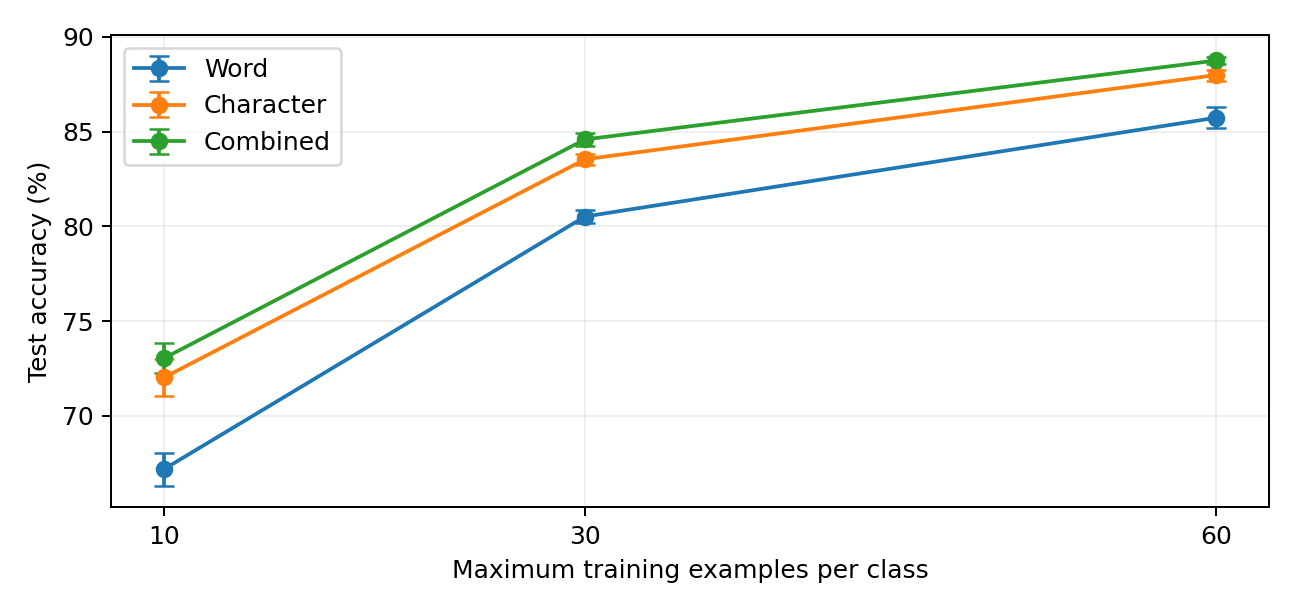
\includegraphics[width=\linewidth]{../results/learning_curve.png}\end{center}
Figure 1. Learning curves with one-standard-deviation error bars. The x-axis is a per-class cap, not a guaranteed count for every class.

The combined representation has the highest mean accuracy at each tested cap and in the pool condition. At cap 10 its advantage over word features is 5.85 percentage points. The gain shrinks as more training data become available. This is consistent with complementary substring information being particularly useful when word statistics are sparse, but does not establish robustness to arbitrary spelling errors.

\clearpage
\subsection*{6.1 Comparison, cost and sensitivity}
For the pool models, combined features improve accuracy by 2.79 percentage points over word features. The paired bootstrap 95\% interval is [2.08, 3.54] percentage points. The interval is unadjusted and applies to this pair of fitted models.

Pool training takes 0.77 s for word features, 1.88 s for character features and 2.43 s for the combination on the measured machine. These are single-run timings, not a rigorous latency benchmark. Removing the seven overlapping test rows leaves 3073 rows and gives 90.89\% combined accuracy; the main conclusion is unchanged in this diagnostic.

\begin{longtable}{p{4.83cm}p{4.83cm}p{4.83cm}}
Method & Training protocol & Accuracy (\%) \\
Word + character SVM (ours) & 7,999 training-pool examples & 90.91 \\
BERT-TUNED [4] & Full official train; published & 93.66 \\
USE + ConveRT [4] & Full official train; published & 93.36 \\
USE + ConveRT [4] & 10 per intent; published & 85.19 \\
\end{longtable}
Table 2. Historical context from [4], Table 3. Neural methods were not rerun. Training budgets, subsets, pretraining and validation protocols differ; these numbers do not constitute a controlled ranking. The combined classifier remains below both full-training neural reference scores.

\subsection*{6.2 Error Analysis}
The combined pool model makes 280 errors. Frequent directional confusions include card arrival versus delivery estimate (4 cases), fiat-currency support versus supported cards/currencies (4), and failed versus reverted top-up (4). Verification-related classes are also confused. These distinctions often depend on the purpose of the request rather than isolated keywords.

\begin{longtable}{p{4.83cm}p{4.83cm}p{4.83cm}}
Test message & True intent & Prediction \\
When will I get my card? & card arrival & card delivery estimate \\
Can I link another card to my account? & card linking & getting spare card \\
Is it a good time to exchange? & exchange rate & exchange charge \\
There is a fee I do not recognize on my statement. & extra charge on statement & card payment not recognised \\
\end{longtable}
Table 3. Actual erroneous predictions; the final message is lightly paraphrased for readability. The full original text and all 280 errors are in results/errors\_combined.csv. The examples show where lexical overlap and missing transaction context make the category distinction difficult.

A lexical representation cannot reliably resolve paraphrases with little shared vocabulary, long-range composition or implicit context. Character features can also amplify irrelevant surface similarity. The error review is qualitative. Separate tests on paraphrases, spelling noise and out-of-domain requests are needed to assess generalization.

\clearpage
\section*{7 Conclusion}
The experiments show that a linear classifier can benefit from combining word and character features for banking-intent classification. Combining word and character TF-IDF with a linear SVM reaches 90.91\% official-test accuracy and outperforms the two single-branch baselines in the tested regimes. The learning curves show a larger benefit over word features when fitting data are scarce. Code, data provenance, predictions and uncertainty diagnostics accompany the report.

The conclusions are limited to one English-language dataset. The capped experiments use three sampling seeds, while the pool condition has a single fit. The next step is to compare the same splits with a frozen sentence encoder and SetFit, then test the models on paraphrases and requests outside the banking domain.

\section*{References}
[1] Sida Wang and Christopher D. Manning. 2012. Baselines and Bigrams: Simple, Good Sentiment and Topic Classification. ACL, pp. 90-94. https://aclanthology.org/P12-2018/

[2] Jacob Devlin, Ming-Wei Chang, Kenton Lee and Kristina Toutanova. 2019. BERT: Pre-training of Deep Bidirectional Transformers for Language Understanding. NAACL-HLT, pp. 4171-4186. https://aclanthology.org/N19-1423/

[3] Nils Reimers and Iryna Gurevych. 2019. Sentence-BERT: Sentence Embeddings using Siamese BERT-Networks. EMNLP-IJCNLP, pp. 3982-3992. https://aclanthology.org/D19-1410/

[4] Inigo Casanueva, Tadas Temcinas, Daniela Gerz, Matthew Henderson and Ivan Vulic. 2020. Efficient Intent Detection with Dual Sentence Encoders. NLP for Conversational AI, pp. 38-45. https://aclanthology.org/2020.nlp4convai-1.5/

[5] Lewis Tunstall et al. 2022. Efficient Few-Shot Learning Without Prompts. arXiv:2209.11055. https://arxiv.org/abs/2209.11055

[6] PolyAI. Task-specific datasets: BANKING77 data and CC BY 4.0 license. Data snapshot retrieved 20 September 2026. https://github.com/PolyAI-LDN/task-specific-datasets

\end{document}